\documentclass[10pt,a4paper]{article}
\usepackage[utf8]{inputenc}
\usepackage[T1]{fontenc}
\usepackage[sfdefault,lining]{FiraSans}
\usepackage[scaled=0.88]{FiraMono}
\usepackage[english]{babel}
\usepackage[margin=2.6cm]{geometry}
\usepackage{graphicx}
\usepackage{placeins}
\usepackage{float}
\usepackage{needspace}
\usepackage{enumitem}
\setlist{itemsep=0.15em, topsep=0.2em, parsep=0pt}  
\usepackage[font=small,labelfont=bf]{caption}
\setlength{\parindent}{0pt}
\setlength{\parskip}{0.6em}
\linespread{1.06}
\setlength{\emergencystretch}{2em}
\widowpenalty=10000
\clubpenalty=10000
\renewcommand{\topfraction}{0.9}
\renewcommand{\bottomfraction}{0.8}
\renewcommand{\textfraction}{0.08}
\renewcommand{\floatpagefraction}{0.85}
\setcounter{topnumber}{3}
\setcounter{totalnumber}{4}

\begin{document}

{\LARGE\bfseries DxO PhotoLab Miniature Effect: notes}\par
{\small 15 November 2026}

\section*{A few observations}

\subsection*{First photo: a landscape, to see what the effect looks like}

We started by applying the effect to an ordinary photo (a lake, a mountain in the background, branches in the foreground), just to see what it does. We tried four blur settings: 0/0, 51/51, 100/100 and 100/0, where the first number is the slider for the top of the image and the second the slider for the bottom.

\begin{figure}[!htbp]
  \centering
  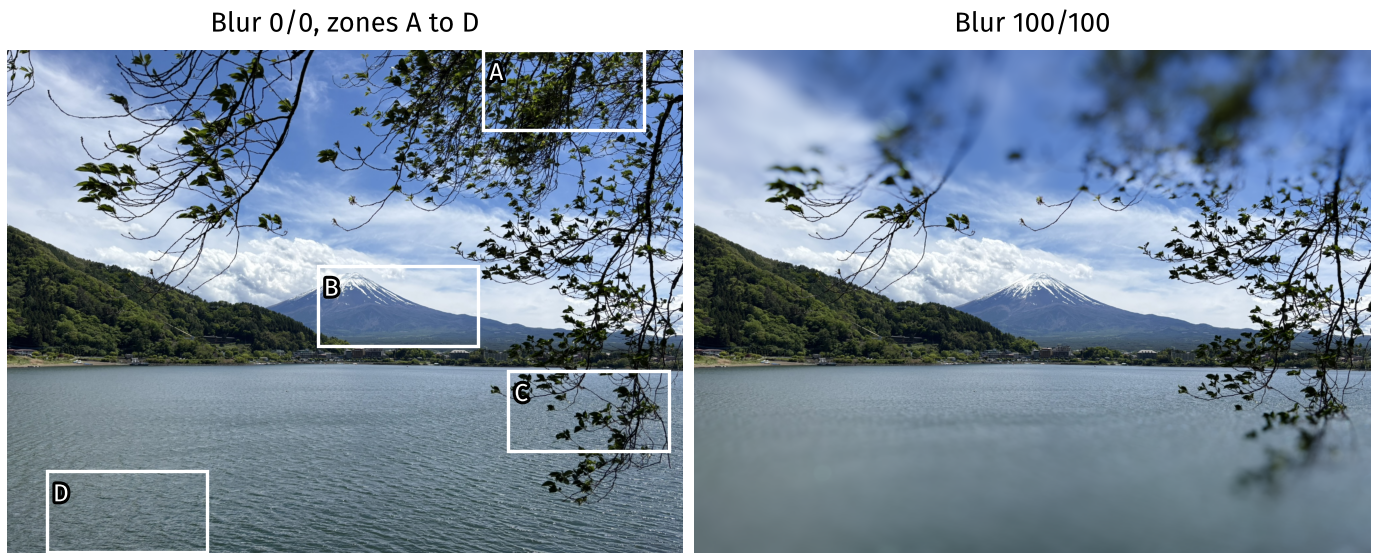
\includegraphics[width=0.88\textwidth]{figures/fig_lake.png}
  \caption{The first photo without blur and with the blur at its maximum. Frames A to D are enlarged in figure~\ref{fig:zones}.}
  \label{fig:lake}
\end{figure}

The blur only affects the top and the bottom of the image. In the middle, a horizontal band stays sharp across the full width, and it is the same for all four settings (zone B in figure~\ref{fig:zones}). The change from sharp to blurred is gradual: in zone C, the upper leaves are sharp, the lower ones blurred, with no visible boundary in between. From 51 to 100, the blur gets stronger but starts at the same place. At 100/0, the bottom is sharp again and the top does not change, so the two sides are set independently.

\begin{figure}[!htbp]
  \centering
  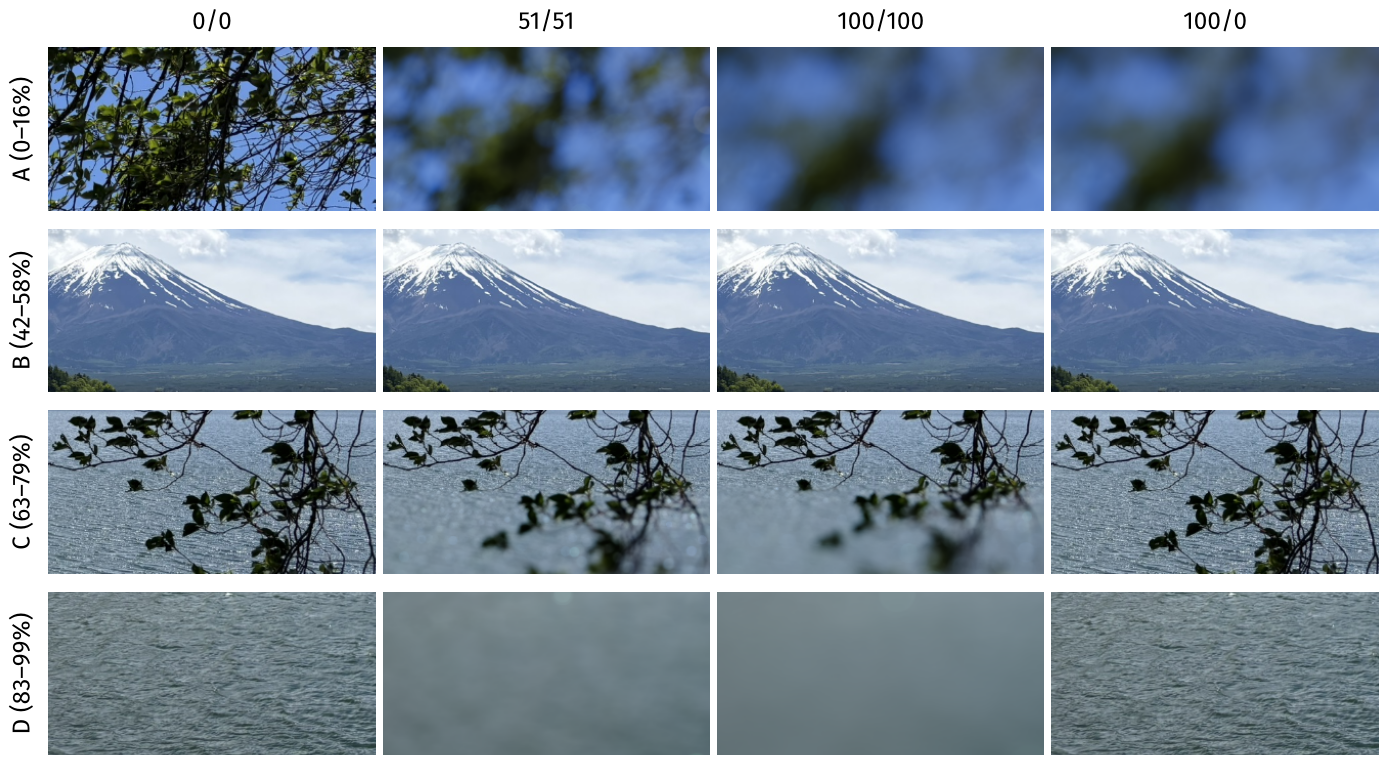
\includegraphics[width=0.84\textwidth]{figures/fig_lake_zones.png}
  \caption{Zones A to D for the four settings. In brackets, the height of each zone in the photo, from 0\% at the top to 100\% at the bottom. For the last setting, the blur shape was also different (9 blades), which does not show at this scale.}
  \label{fig:zones}
\end{figure}

The most interesting part is the branches on the right. They are all in the foreground, and yet they are sharp inside the band and blurred above and below it. Conversely, at a given height everything is blurred in the same way, the lake as well as the leaves or the sky. That is also why the miniature look only half works on this photo: the bottom is convincing, since the lake gets closer as you go down, but at the top the sky is blurred while branches that are very close stay sharp.

On the other hand, this photo says almost nothing about the shape of the blur. The only clue is that at 51/51 the sun's reflections on the lake turn into small pale discs. To study that shape we need isolated points of light, hence the second photo.

\FloatBarrier
\subsection*{Second photo: a night view, to see the shape of the blur}

For this second test, we pick a photo that suits the effect better, an aerial night view (Tomáš Galbavý, Unsplash, 4000~×~3000 pixels). Each lamp is almost a point of light on a dark background, so what it turns into after the effect shows directly how a point is blurred. We exported several JPEG versions, changing only one setting at a time, and we keep four of them: N00 without the effect, N01 with the blur at 50, N02 with the blur at 100, and N05 with the blur at 100 and the ``6 blades'' shape instead of ``Circular''.

In PhotoLab, the tool displays four lines on the photo (figure~\ref{fig:night}, right): two solid lines in the middle and two dashed lines further out. With the default settings, the solid lines are at about 30\% and 70\% of the height of the image, and the dashed ones at about 10\% and 90\%, counting 0\% at the very top.

\begin{figure}[!htbp]
  \centering
  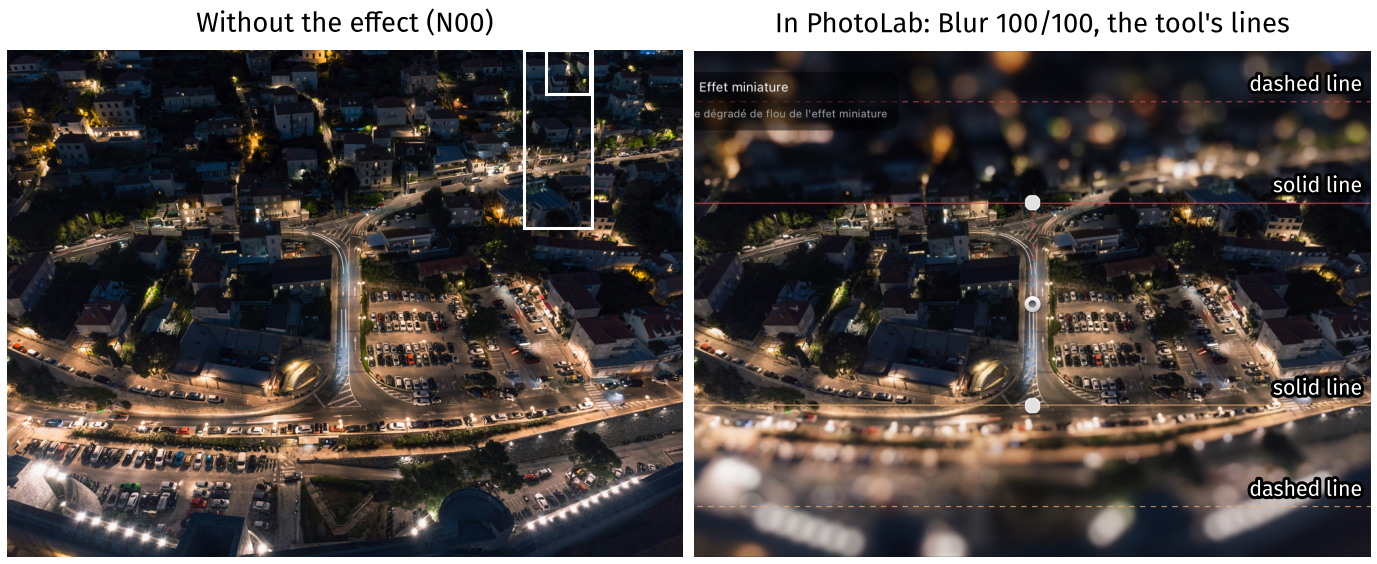
\includegraphics[width=0.92\textwidth]{figures/fig_night.png}
  \caption{Left, the night photo without the effect. The large frame is the strip of figure~\ref{fig:strips}, and the small square inside it is the lamp of figure~\ref{fig:lamp}. Right, a PhotoLab screenshot with the blur at 100 on both sides and the four lines of the tool (the banner at the top left is part of PhotoLab's display).}
  \label{fig:night}
\end{figure}

Between the two solid lines, N02 cannot be told apart from N00. Above them (figure~\ref{fig:strips}), the blur appears at the solid line, increases steadily up to the dashed line, then stops increasing all the way to the edge. At Blur 50 (N01), the zones are the same and the blur is weaker everywhere.

\begin{figure}[!htbp]
  \centering
  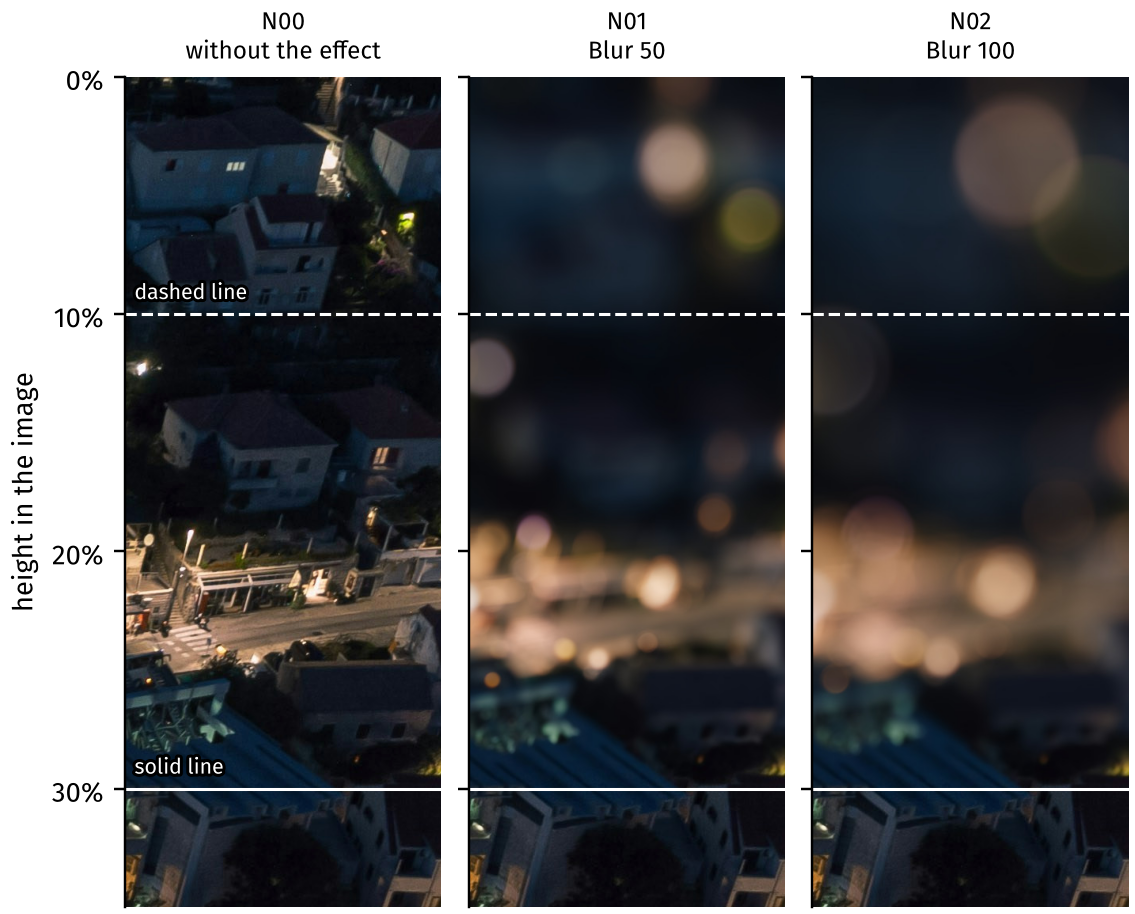
\includegraphics[width=0.58\textwidth]{figures/fig_strips.png}
  \caption{The same vertical strip of the photo (large frame of figure~\ref{fig:night}), from the top edge down to 35\% of the height, in three exports. The two upper lines of the tool are drawn in white.}
  \label{fig:strips}
\end{figure}

Each lamp turns into a round spot, of the same color as the lamp. The further the lamp is from the solid line, the bigger its spot, and the spots are clearly smaller at Blur 50 than at Blur 100.

Zooming in on one lamp (figure~\ref{fig:lamp}), we can see that the spot has a sharp edge: it is a disc, not a glow that fades out little by little. And when we pick ``6 blades'' in the Shape menu, this disc becomes a hexagon.

\begin{figure}[!htbp]
  \centering
  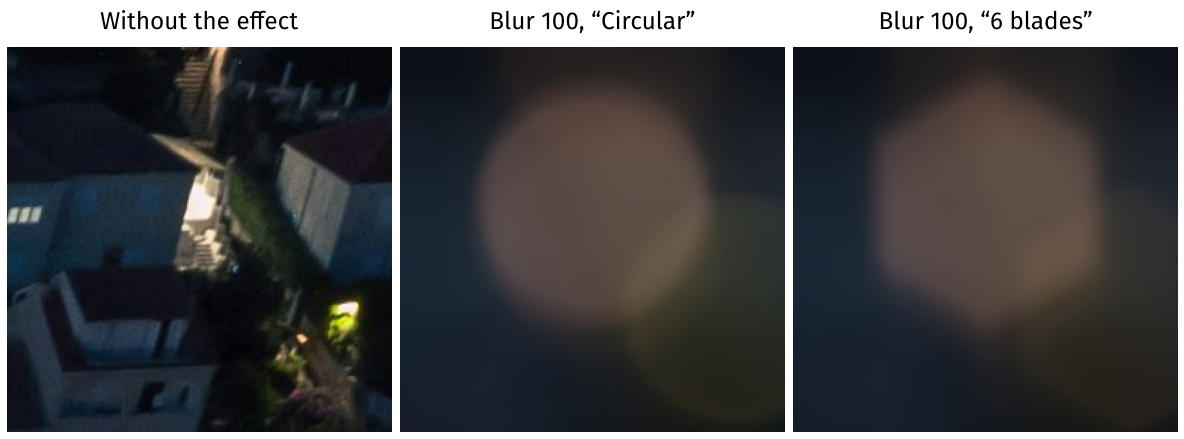
\includegraphics[width=0.66\textwidth]{figures/fig_lamp.png}
  \caption{Zoom on one lamp (small square of figure~\ref{fig:night}, 260~×~260 pixels): without the effect, then with the blur at 100 for two shapes.}
  \label{fig:lamp}
\end{figure}

All this shows what the effect does, but not how it does it. We are left with three questions:

\begin{enumerate}
  \item What decides how much blur there is at a given place in the image?
  \item How does this blur grow as we move away from the sharp band?
  \item What exactly does a point of light turn into, and what does the Blur slider set?
\end{enumerate}

\FloatBarrier
\needspace{10\baselineskip}
\section*{Hypotheses}

One hypothesis per question. Each time, we recall what we observed, say what we assume, then what we should see on a test image if it is true.

\begin{enumerate}
  \item On the lake photo, the same branch is sharp inside the band and blurred above it. So we assume that the blur only depends on where we are in the image, and not on what is in it. If that is true, a checkerboard, which is nothing like a photo, should show the same sharp band and the same blurred zones.

  \item On both photos, the blur increases little by little as we move away from the band. We assume that there is no blur at all between the two solid lines, that the blur grows from the solid line up to the dashed line, and that it then stays the same all the way to the edge. This is also what DxO's help says\footnote{\texttt{userguides.dxo.com/en/viewpoint/tools}, section ``Miniature Effect''.}, but we want to check it ourselves. If that is true, on a column of identical white discs, the discs inside the band should stay intact, then the spots should get bigger and bigger, then all be the same.

  \item On the night view, each lamp turns into a round spot, smaller at Blur 50 than at Blur 100. We assume that each point is spread into a disc, and that the size of this disc is proportional to the Blur slider. If that is true, a single white disc on a black background should turn into a bigger disc with a sharp edge, about half as big at Blur 50 as at Blur 100.
\end{enumerate}

\section*{Test images}

To test these hypotheses, we need very simple images in which we know every pixel. We made four with \texttt{code/make\_test\_images.py} (folder \texttt{test\_images/}, figure~\ref{fig:test}). They are all 4000~×~3000 pixels like the night photo, and they are TIFF files, because a JPEG would damage the image before the blur is even applied:

\begin{itemize}
  \item \texttt{gray.tif}: a uniform gray. It is the control, it should not change.
  \item \texttt{checkerboard.tif}: a black and white checkerboard with 50-pixel squares (hypothesis 1).
  \item \texttt{column.tif}: a column of 15 identical white discs on black, one every 200 pixels from top to bottom (hypothesis 2). With the default settings, there is a disc on each of the four lines.
  \item \texttt{disc.tif}: just one of these discs, about twenty pixels wide, at the top of the image, where the blur is strongest (hypothesis 3).
\end{itemize}

\begin{figure}[!htbp]
  \centering
  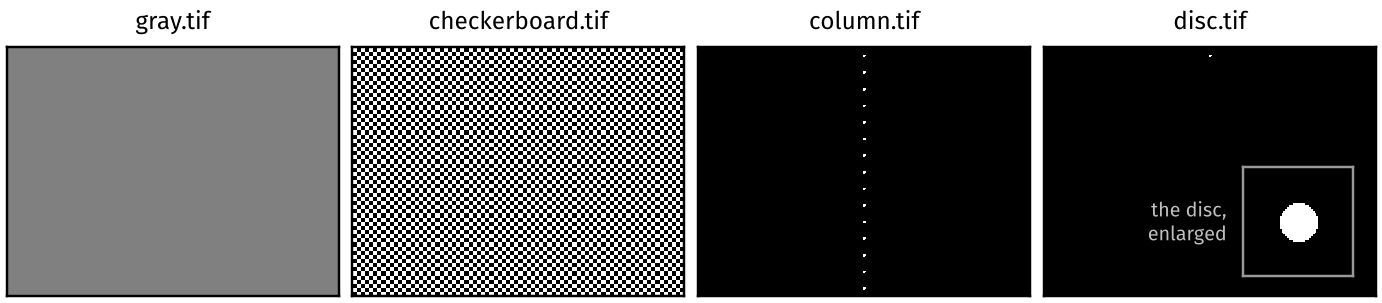
\includegraphics[width=0.86\textwidth]{figures/fig_test_images.png}
  \caption{The four test images. The discs are tiny at this scale, the one in \texttt{disc.tif} is enlarged in the corner.}
  \label{fig:test}
\end{figure}

For the tests, we will always do the same thing. We first apply the ``6 - No correction'' preset, as the assignment asks, we write down what we expect to see, then we export, changing only one setting at a time. First each image without the effect, to check that it comes out identical. Then the gray, the checkerboard and the column with the blur at 100, then the disc with the slider at 25, 50, 75 and 100, and finally the column after moving one line. That makes about a dozen exports. For each hypothesis, we will conclude that it holds, that it does not hold, or that it only holds in some cases.

\end{document}
